\begin{tikzpicture}
	\begin{axis}[
		name=plot1,
		xlabel={$\eta_1$},
		ylabel={$\eta_2$},
		font = \scriptsize,
		width=0.5\textwidth,
		height=0.35\textwidth, %height= 5/3*0.5
		ytick pos=left,
		xtick pos=top,
		line width = 0.85pt,
		]
		% \addplot [color = blue,mark =x,only marks] table [x expr=\thisrow{eta1}, y expr = \thisrow{eta2}]{\myGraphs/etaData/eta_num/eta_0.csv};
		\addplot [color = blue,mark =none] table [x expr=\thisrow{eta1}, y expr = \thisrow{eta2}]{\myGraphs/etaData/eta_num/eta_1.csv};
		% \addplot [color = red,mark =x,only marks] table [x expr=\thisrow{eta1}*100, y expr = \thisrow{eta2}*100]{\myGraphs/etaData/eta_num/eta_exp/eta_0.dat};
		\addplot [color = red,mark =none] table [x expr=\thisrow{eta1exp}, y expr = \thisrow{eta2exp}]{\myGraphs/etaData/eta_num/eta_1.csv};
		% \addplot [color = red,mark =none] table [x expr=\thisrow{x}, y expr = \thisrow{singValsqLomSumasingValsq}]{\myGraphs/singValsData/singVals_U_exp.dat};
	\end{axis}

	\matrix[
		matrix of nodes,
		anchor=south,
		draw,
		inner sep=0.2em,
		font = \scriptsize,
		%~ thick,
		fill=white,
	]at([xshift=0.2cm,yshift=0.4cm]plot1.north east)
	{
		%~ \ref{100}& CFD old &[5pt]\\
		%~ \ref{60}& XPF - reac, wall&[5pt]\\
		\ref{expSigm}& PIV &
		\ref{numSigm}& CFD &
		\\
	%        \ref{legendNoReact}& $\mathrm{thermic\ no\ reaction\ heat}$&[5pt]
		\\};
	\begin{axis}[
		anchor = north west,
		at = {(plot1.north east)},
		xlabel={$\eta_{15}$},
		ylabel={$\eta_{16}$},
		font = \scriptsize,
		name=plot2,
		% xtick distance=1,ytick distance=1,
		width=0.5\textwidth,
		height=0.35\textwidth, %height= 5/3*0.5
		xshift=0.03\textwidth,
		% x label style = {at={(axis cs:3.5,-2.7)}},
		% y label style = {at={(axis cs:-1,0)}},
		% enlargelimits=false,
		% scale only axis=true,
		ytick pos=right,
		xtick pos=top,
		% ymode=log,
		% xmode=log,
		line width = 0.85pt,
		% xmax=2000,
		% xmin=1,
		% ymax=1,
		% ymin=1e-5,
		%  tick align=outside,
		]
		\addplot [color = blue,mark =none] table [x expr=\thisrow{eta15}, y expr = \thisrow{eta16}]{\myGraphs/etaData/eta_num/eta_1.csv};
		\addplot [color = red,mark =none] table [x expr=\thisrow{eta9exp}, y expr = \thisrow{eta10exp}]{\myGraphs/etaData/eta_num/eta_1.csv};
		% \addplot [color = red,mark =none] table [x expr=\thisrow{eta15exp}*1000, y expr = \thisrow{eta16exp}*1000]{\myGraphs/etaData/eta_num/eta_1.csv};
		% \addplot [color = red,mark =none] table [x expr=\thisrow{eta3}*100, y expr = \thisrow{eta4}*100]{\myGraphs/etaData/eta_num/eta_exp/eta_0.dat};
	\end{axis}

	\savebox\mygraphic{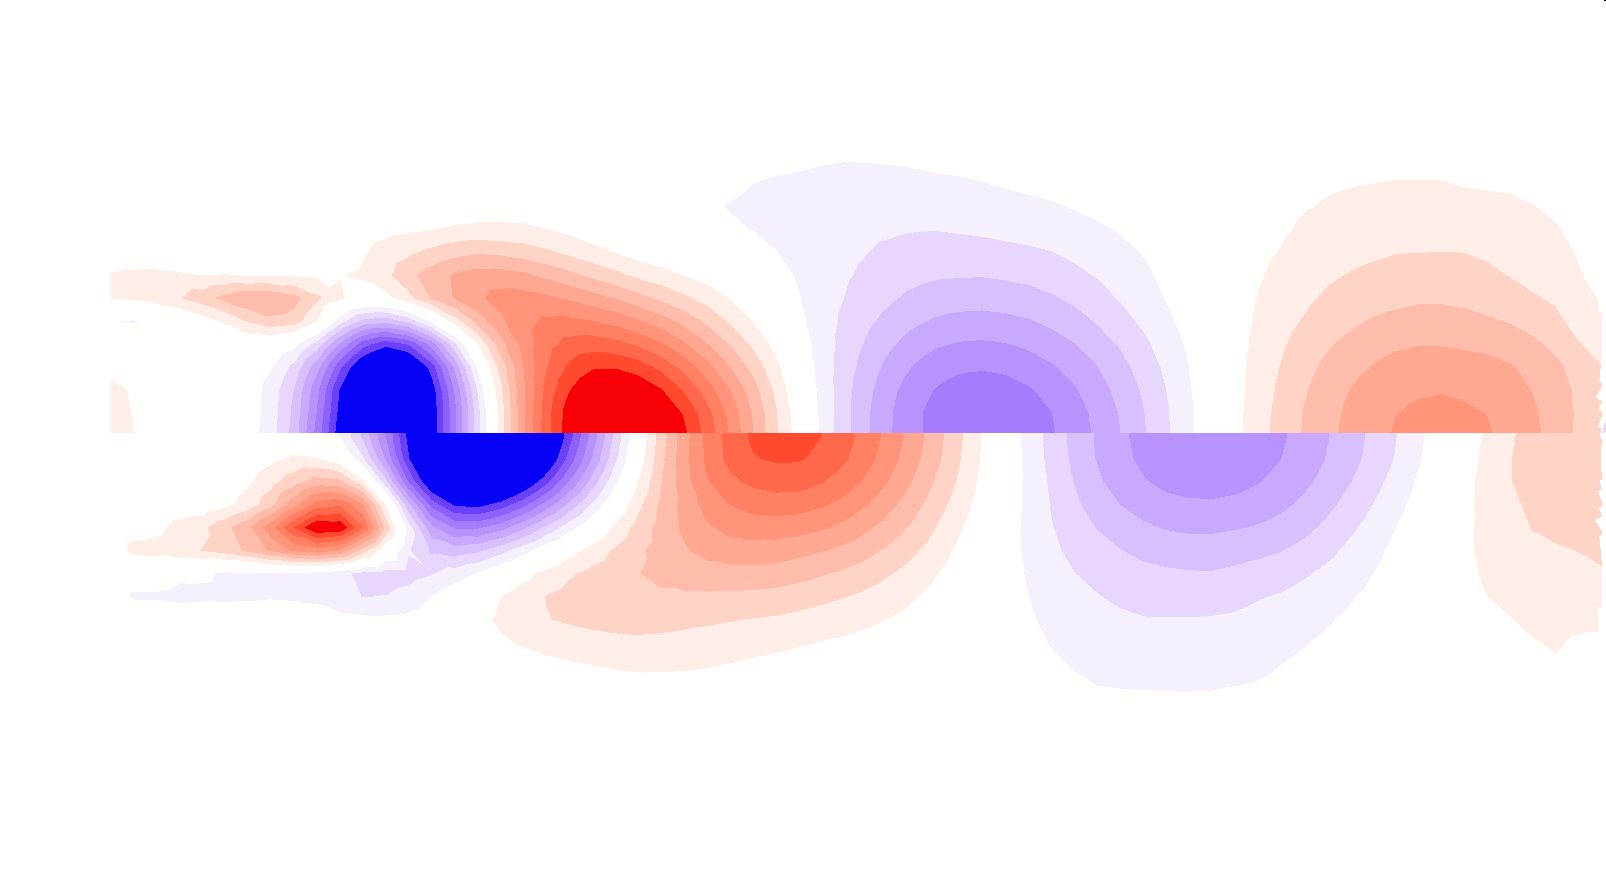
\includegraphics[trim = 0px 0px 0px 0px,clip,width = 0.37\textwidth]{\myImages/mods/exp/mod1mod2.png}}
	\begin{axis}[
		at = {(plot1.south west)},
		anchor=north west,
		name = plot3,
		yshift=-0.03\textwidth,
		xlabel={$x_r$ [-]},
		ylabel={$y_r$ [-]},
		font = \scriptsize,
		xtick distance=1,ytick distance=1,
		width=\wd\mygraphic,
		height=\ht\mygraphic, %height= 5/3*0.5
		enlargelimits=false,
		scale only axis=true,
		tick align=outside,
		ytick pos=left,
		xtick pos=bottom,
		x label style = {at={(axis cs:1,-2.7)}},
		line width = 1.7pt
		]
		\addplot graphics[xmin=0, xmax=7, ymin=-2, ymax=2,includegraphics={trim = 0px 0px 0px 0px,clip}] {\myImages/mods/exp/mod1mod2.png};
		\fill [white] (axis cs:0.001,-1.997) rectangle (axis cs:0.5,1.997);
		\fill [black!70](axis cs:0,0) circle [radius=0.5];
		\draw [black,dashdotted,line width = 1pt] (axis cs:0,0) -- (axis cs:7,0);

		% \node at (axis cs:6.5,-1.7) {\scriptsize{CFD}};
		% \draw [black!70,dashed,line width = 1pt] (axis cs:3.83,2) -- (axis cs:3.83,-2);
		% \node [black!70] at (axis cs:4.1,1.7) {\scriptsize{$\zeta$}};
	\end{axis}
	\node[anchor=north east] at (plot3.north east) {\scriptsize{mode 1}};
	\node[anchor=south east] at (plot3.south east) {\scriptsize{mode 2}};

	\savebox\mygraphic{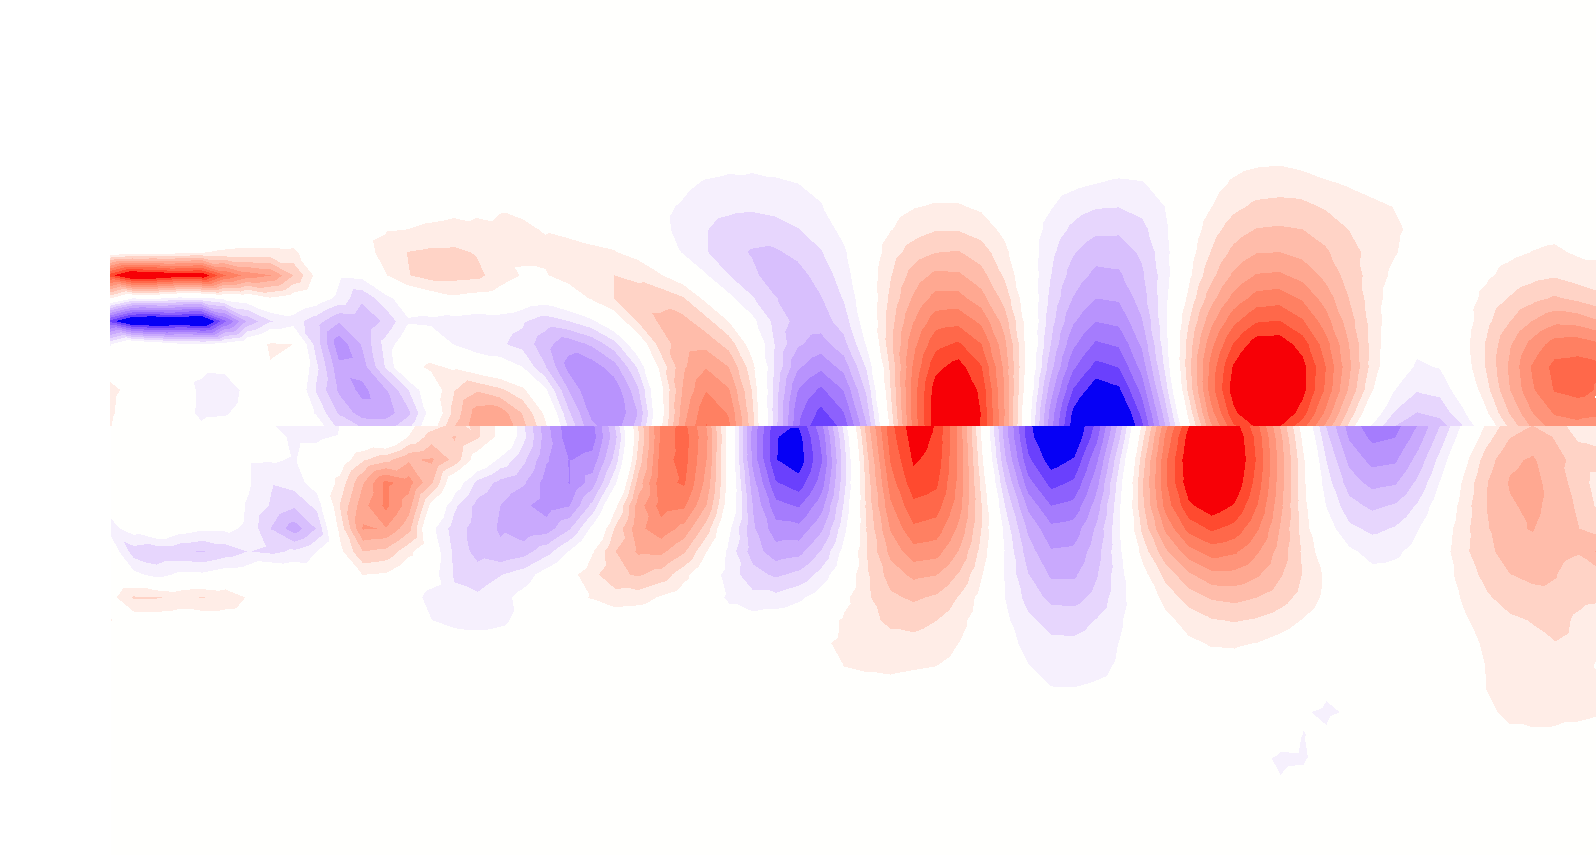
\includegraphics[trim = 0px 0px 0px 0px,clip,width = 0.37\textwidth]{\myImages/mods/exp/mod15mod16.png}}
	\begin{axis}[
		at = {(plot2.south west)},
		anchor=north west,
		name = plot4,
		yshift=-0.03\textwidth,
		xlabel={$x_r$ [-]},
		ylabel={$y_r$ [-]},
		font = \scriptsize,
		xtick distance=1,ytick distance=1,
		width=\wd\mygraphic,
		height=\ht\mygraphic, %height= 5/3*0.5
		enlargelimits=false,
		scale only axis=true,
		tick align=outside,
		ytick pos=right,
		xtick pos=bottom,
		line width = 1.7pt,
		x label style = {at={(axis cs:6,-2.7)}},
		]
		\addplot graphics[xmin=0, xmax=7, ymin=-2, ymax=2,includegraphics={trim = 0px 0px 0px 0px,clip}] {\myImages/mods/exp/mod15mod16.png};
		\fill [white] (axis cs:0.001,-1.997) rectangle (axis cs:0.5,1.997);
		\fill [black!70](axis cs:0,0) circle [radius=0.5];
		\draw [black,dashdotted,line width = 1pt] (axis cs:0,0) -- (axis cs:7,0);
		% \node at (axis cs:6.5,-1.7) {\scriptsize{CFD}};
		% \draw [black!70,dashed,line width = 1pt] (axis cs:3.83,2) -- (axis cs:3.83,-2);
		% \node [black!70] at (axis cs:4.1,1.7) {\scriptsize{$\zeta$}};
	\end{axis}
	\node[anchor=north east] at (plot4.north east) {\scriptsize{mode 15}};
	\node[anchor=south east] at (plot4.south east) {\scriptsize{mode 16}};
	\node [name = osaUx,anchor = south east,at={(plot3.south east)},yshift=-0.8cm,xshift=0.2\textwidth] {
\includegraphics[width=0.3\textwidth]{\myImages/res/vorZ_scale.png}};
	\node [name = vorZ, anchor = east,at={(osaUx.north west)},yshift=-0.3cm,xshift=0.0cm] {\scriptsize{$\omega_z$ [-]}};
	\node [name = psi0, anchor = south,at={(osaUx.north)},yshift=-0.6cm,xshift=-1.3cm] {\scriptsize{negative}};
	\node [name = psi0, anchor = west,at={(psi0.east)},yshift=-0.0cm,xshift=1.4cm] {\scriptsize{positive}};
\end{tikzpicture}